\documentclass[a4paper,12pt]{article}

\usepackage{graphicx}
\usepackage[hidelinks]{hyperref}
\usepackage{multibib}
\usepackage{fancyhdr}
\usepackage{listings}
\usepackage{float}

\usepackage{tikz}
\usetikzlibrary{arrows,automata,positioning,matrix}
\usepackage[pdftex]{pict2e}
\usepackage[top=1.25in,bottom=1.25in,left=1.5in,right=1.25in]{geometry}

\fancyhf{} % clear all header and footers
\renewcommand{\headrulewidth}{0pt} % remove the header rule
\rfoot{\thepage}

\newcites{bib}{Bibliography}
\newcites{ref}{References}
\bibliographystyle{apalike}


\pagestyle{fancy}
\begin{document}
\nociteref{*}
\nocitebib{*}
\setcounter{secnumdepth}{4} %so that we get subsubsubsection
\setcounter{tocdepth}{4} %so that subsubsubsection get's shown on Table of contents

\begin{center}
    \pagenumbering{gobble}
    \textbf{\Large Kathmandu University} \\[0.3cm]
    \textbf{\large Department of Computer Science and Engineering} \\[0.3cm]
    \textbf{\Large Dhulikhel,Kavre} \\[0.8cm]

    
\includegraphics[width=0.3\textwidth]{images/ku.jpg} \\[0.6cm]


    \textbf{\large A Project Report} \\[0.3cm]
    \textbf{\large on} \\[0.6cm]
    { \huge \bfseries “FPGA Console”} \\[0.3cm]

    { \large \bfseries COMP 342} \\[0.3cm]

    { \normalsize \bfseries for  partial fullfullment of III/II in Computer Science/Engineering} \\[0.6cm]

    \textbf{\large Submitted By} \\[0.2cm]

    \textbf{\large Ashish Thapa(56)}

    \textbf{\large Aditya Jha(20)} \\[1.2cm]

    \textbf{\large Submitted To} \\[0.2cm]
    \textbf{\large Dr. Rajani Chulyadyo} \\[0.2cm]
    \textbf{\large Department of Computer Science and Engineering} \\[1.5cm]


    \textbf{\large Submission Date:} \\[0.3cm]
    \today
\end{center}

    \newpage
    \vspace*{2cm}
    \begin{center}
    \section*{Bonafide Certificate}
    \pagenumbering{Roman}
    \addcontentsline{toc}{section}{Bonafide Certifate}
    \vspace{2cm}
    \textbf{\large This project Work on} \\[0.2cm]
    \textbf{\large “FPGA Console”} \\[0.2cm]
    \textbf{\large is the bonafide work of} \\[0.2cm]
    \textbf{\large “Ashish Thapa, Aditya Jha”} \\[0.2cm]
    \textbf{\large who carried out the project work under my supervision} \\[0.2cm]
    \end{center}

    \vspace{3cm}
    \phantom{} \\[0.2cm]
    \textbf{\large Project Supervisor}
    \phantom{} \\[0.2cm]
    \rule{6cm}{0.1pt} \\[0.2cm]
    \textbf{\large Name: Dr. Sudan Jha} \\[0.2cm]
    \textbf{\large Academic Designation: Professor}

    \newpage
    \section*{Abstract}
    \addcontentsline{toc}{section}{Abstract}


    FPGA technology has been widely used in digital systems, especially in embedded systems. Tang Nano 9k is a low-cost FPGA board that can be used to implement digital systems. The aim of this project is to create a custom CPU focused to act as a brain for a game console using Tang Nano 9k FPGA board. This project aims to provide hands-on experience with FPGA development and custom ISA implementation.The project uses open source tools for digital design like Yosys,synth\_gowin,next pnr-gowin,iverilog, GTKWave etc. The project includes the development of a CPU with a custom ISA, buttons as  input device, SSD1306 OLED as a output device, and ESP8266 as a display controller. Various protocols like UART, SPI, and I2C are used to communicate with various modules within the fpga console. The outcome of this project is a working game console where assembly code for games like pong can be loaded into the flash and played. The project has provided a better understanding of communication interface, fpga toolchain and implementation of custom ISA.This project can be extended to include more advanced features such as networking capabilities, sound output, and additional input devices. 
    \vspace{0.5cm}

    \noindent
    \textbf{Keywords}: \textit{FPGA technology, game console,, Yosys, nextpnr-gowin, GTKWave, custom CPU, ,UART, SPI, assembly}

    \newpage
    \pagenumbering{gobble}
    \tableofcontents

    % defining list of figures and list of tables

    \newpage
    \listoffigures
    \addcontentsline{toc}{section}{List of Figures}
    \pagenumbering{Roman}
    \setcounter{page}{3}

    \newpage
    \listoftables
    \addcontentsline{toc}{section}{List of Tables}
    \newpage

    % abbreviation

    \section*{Abbreviation} 
    \addcontentsline{toc}{section}{Abbreviation}
    \renewcommand{\arraystretch}{2.3}
    \label{tab:acronyms}
    \begin{tabular}{|c|p{0.7\linewidth}|}
    \hline
    \textbf{Acronym} & \textbf{Description} \\
    \hline
    FPGA & Field-Programmable Gate Array \\
    ISA & Instruction Set Architecture \\
    OLED & Organic Light Emitting Diode \\
    ESP & Electronic Stability Program \\
    UART & Universal Asynchronous Receiver-Transmitter \\
    SPI & Serial Peripheral Interface \\
    I2C & Inter-Integrated Circuit \\
    CPU & Central Processing Unit \\
    VGA & Video Graphics Array \\
    HDL & Hardware Description Language \\
    DSA & Domain Specific Architecture\\
    RISC & Reduced Instruction Set Architecture\\
    CISC & Complex Instruction Set Architecture\\
    ASIC & Application Specific Integrated Circuit\\
    \hline
    \end{tabular}

    % main matter
    \newpage
    \pagenumbering{arabic}
    \setcounter{page}{1}
    \section{Introduction}
    \subsection{Background}

    \phantom{}

    Field Programmable Gate Arrays (FPGA) are integrated circuits that can be programmed to perform any digital function by configuring the interconnects and logic gates inside the chip. They are different from processors or microcontrollers as FPGA contains logic blocks and look up tables that are placed and routed , which means there is no instruction set and fetching, decoding or executing. It can be optimized for specific tasks and it allows parallel processing .Since its inception in Xilinx has seen rapid growth and adoption mainly because of its high configurability and flexibility. 

    Since FPGA performance is comparable to real digital circuit, and the toolchain it comes bundled with allows easy testing and prototyping. Building the CPU with custom Instruction set becomes relatively easy. A CPU has a predefined set of instructions one can use to program it. Those instructions or Instruction set architecture are of two types i.e  Complex Instruction Set Architecture(CISC) and Reduced Instruction Set Architecture(RISC). RISC has limited number of instruction set and simpler microarchitecture. RISC-V contains 32-bit integer instruction set called \textbf{RV32I}, which includes 47 instructions only \citebib{arvindpdmn_risc-v_2018}. Other Popular Instruction set architectures are x86, ARM , MIPS, Xtensia etc. 

    Gaming Consoles have been around 1970s and has evolved significantly over the years. The first game console, Magnavox Odyssey, was released in 1972 was a simple analog device. Today consoles like PS5, Xbox, Nintendo Switch are sophisticated devices with advanced features. %%\citebib{cite world history here} %.
    The project aim is to create a simple enough game console using an FPGA which offers flexibility and customization. This approach allows us total control over how the console is designed. The Instruction set architecture can be specifically designed to cater console devices. 

    \subsection{Objectives}
    \begin{itemize}
        \item To create a simple game console using the FPGA, with simple input and output devices.
        \item To Design and implement our own CPU with custom Instruction Set Architecture(ISA) which can be used to write the games for the console
        \item To understand and use various hardware communication interfaces like UART, SPI , $I^2C$
        \item To develop proficiency in programming with Hardware Description language(HDL) like Verilog  
    \end{itemize}

    \subsection{Motivation and Significance}
    FPGAs are highly versatile programmable devices which can perform any digital function. It also generally supports large array of input/output pins which can interface with other deivces. The motivation for this project is to create a custom game console from scratch using FPGA technology, with a focus on developing a CPU with a custom instruction set architecture (ISA) and implementing it in hardware. 

    Learning to create a game console or any hardware system from scratch is arduous task. Newer ones are very complex and the old ones or the simple ones either have a closed system architecture or requires different Integrated Circuits(ICs) which are already discontinued to be produced. For those who wants to understand how simple consoles work, there is no proper resources available. This project aims to be as simple as possible and include bare minimum number of input devices, some form of video output while documenting each and every significant part of the process. By creating a custom game console, this project provides a platform for hardware enthusiast to experiment and create new games with a custom instruction set architecture while utilizing parallelization of FPGAs.

    This project is different from existing works in that it focuses on creating a custom game console from scratch, rather than modifying an existing system. Additionally, the development of a custom ISA allows for greater flexibility and optimization of game code. The use of FPGA technology also provides the ability to modify and upgrade the hardware, enabling the console to evolve over time.

    Overall, the significance of this project lies in its potential to inspire further innovation in the field of hardware world, as well as its educational value in providing hands-on experience with FPGA technology, computer architecture, and digital circuit design.
    \newpage
    \section{Related Works}
    \subsection{Architectures}
    Starting From the 1960s, when IBM had 4 computer lines, all of them had 4 different ISAs. Custom instruction set for each computer line which had similar task was not optimal so companies moved towards a standarizing a single instruction set architecture. Intel has x86 architecture, Softbank Group owns ARM architecture, University of California Berkely manages RISC-V architecture. These exisiting architecures represents culmination of years of development and is suitable for various kinds of tasks.
    Custom Instruction set Design also has gained considerable attention in recent years. As the increasing demands for performance arises. Custom design gives total control. One example of Domain specific Architecture (DSA) is Google \textit{ Tensor Processing Unit} first deployed in 2015. 
    \subparagraph{RISC-V}
    It is one of the opensource General purpose specification that can run operating systems, compilers and so on. It has a modular architecture.It supports little endian byte ordering system. Its primary features are
    \begin{itemize}
        \item  completely open ISA which is free to academia and industry.
        \item 32-bit and 64-bit address space variants
        \item support for highly-parallel multicore or manycore implementation
    \end{itemize}
    \subparagraph{ARM}
     architecture is owned by Softbank group. First arm processor called ARM1 was developed by Acord computer in Britain for BBC. The architecture state for the ARM processor consists of 16 \textit{32-bit} registers and the status register. In 1995 it introduced the \textit{16-bit} thumb instruction set which makes the code size small but are less powerful.Later enhancement has added digital signal processing (DSP), optional floating point instructions, power saving and Single instruction Multiple data (SIMD) instructions. ARMv8 introduced a completely new 64-bit architecture. 

    \subparagraph{Google TPU}
    can run \textit{Deep Neural Network} interface 15-to-30 times faster  than contemporary CPU and GPU. %\citebib{}. 
    It can achieve such performance because
    \begin{itemize}
        \item it has large 2-dimensional multiply units compared to contemporary CPU which has 13 to 18 times smaller multiply units.
        \item it uses domain specific architecture (DSA) specifically created to decrease the cost and increase the performance. 
    \end{itemize}

    \subsection{Consoles}

    \subsubsection{Mister FPGA Project}
    Mister is an open source project that aims to recreate classic computers, video game consoles, and arcade machines using modern hardware. It uses an FPGA board called DE10-Nano which connects to TV or monitor via HDMI video out. It can also be expanded with various add-on boards such as 7-port USB hub.

    \begin{figure}[h]
    \centering
    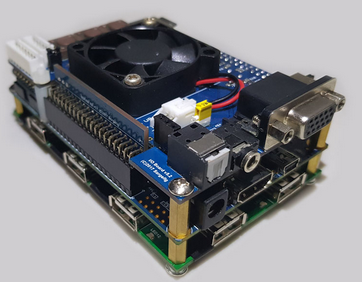
\includegraphics[width=0.5\textwidth]{images/mister.png} 
    \caption{Mister FPGA DE10-Nano Board}
    \end{figure}

    \subsubsection{FPGA-CHIP8} 
    CHIP-8 is a virtual machine with an interpreted environment widely used in the 1970s.
    FPGA-CHIP8 implements CHIP-8 specification for TinyFPGA BX board. Other hardware components are a 16-button keyboard and 128x64px monochrome OLED screen
    \begin{figure}[H]
    \centering
    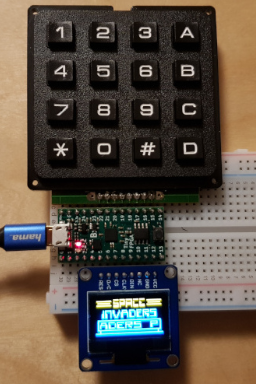
\includegraphics[width=0.3\textwidth]{images/chip8-fpga.png} 
    \caption{FPGA-CHIP8 running Space invaders}
    \end{figure}

    \subsubsection{FPGAboy} 
    FPGABoy is an implementation of Nintendo's classic handheld Game Boy system. It runs on Digilent Atlys board. Xilinx ISE webPACK is used as IDE and for simulations
    \begin{figure}[h]
    \centering
    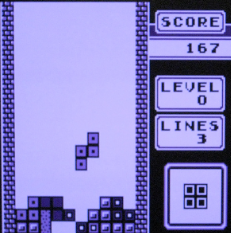
\includegraphics[width=0.3\textwidth]{images/fpgaboy.png} 
    \caption{Tetris run on FPGAboy}
    \end{figure} 
    \newpage
    \section{Design and Implementation}
    \subsection{Procedure}

    \subsubsection{Learning oss-cad-suite}
    OSS CAD Suite is distribution for open source software used in digital logic design.
    There are tools for RTL synthesis, hardware verification, place and route and support for Hardware Definition Language(HDL) like Verilog. HDLBits is collection of verilog exercises suited for learning Verilog. \url{https://hdlbits.01xz.net/wiki/Special:VlgStats/216F4A6FBFA9331} contains the list of solved problems. \textit{Yosys} is the synthesis tool which converts the high level description of design into optimized gate-level netlist. Netlist is list of electric component in a circuit and a list of nodes they are connected to.
    
    \textit{Nextpnr-gowin} is used for place and route. Place and route is the stage of FPGA which takes a \textit{constraint} file and the synthesized file and then decides where to place and route them according to FPGA type. Constraint files are special files which defines the relation between the pins and module input and output variables and then decides where to place and how to route them. \textit{gowin\_pack} is used for Bitstream generation. \textit{OpenFPGALoader} is used to load burn the generated bitstream into the FPGA .
    
    \begin{figure}[H]
        \centering
        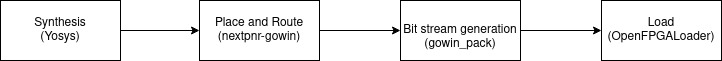
\includegraphics[width=1\textwidth]{./images/oss-process.jpeg}
        \caption{Process of loading HDL Code to FPGA using OSS tools}
    \end{figure}

    \subsubsection{Learning Communication Interfaces and Protocols}
    Communication interfaces defines the set of protocols, and communication channels that allows devices to exchange data or signals with each other. 

    \paragraph{Interfacing with flash memory with SPI interface}
    
    The flash chip used by the FPGA is \textit{P25Q32U} which uses SPI protocol. Serial Peripheral Interface(SPI) is synchronous serial communication interface commonly used for short-distance communication. There are four lines \textit{SCK} ,\textit{Master Out Slave In(MOSI)},\textit{Master In Slave Out(MISO)} and \textit{ChipSelect(CS)}. 

    \begin{figure}[H]
        \centering
        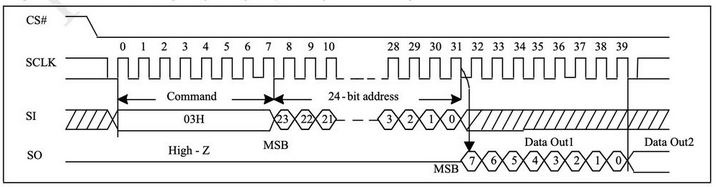
\includegraphics[width=1\textwidth]{./images/spi_flash.png}
        \caption{SPI Read Sequence Timing Diagram for Tang Nano 9k}
    \end{figure}

    Using verilog, SPI state machine was created. There needs to be certain delay time to accomodate for the speed difference between FPGA and the chip itself. The The states are shown by \textit{figure 6}. Each node has \textit{$input/output$} representation. Input section defines the path to take, i.e if past output was 0 then current node will take the path that has \textit{$0/X$} as the input. 

     \begin{figure}[h!]
    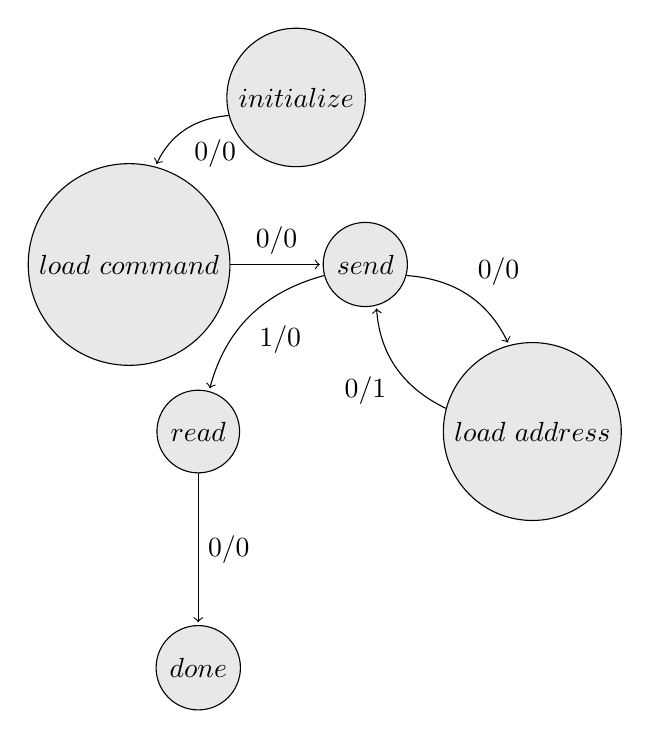
\begin{tikzpicture}[shorten >=1pt,node distance=3cm,auto]
    \tikzstyle{every state}=[fill={rgb:black,1;white,10}]

    \node[state]   (init)                      {$initialize$};
    \node[state] (loadcmd) [below left of=init]  {$load\ command$};
    \node[state]           (send) [right of=loadcmd]     {$send$};
    \node[state] (loadaddr) [below right of=send] {$load\ address$};
    \node[state]           (read) [below left of=send]     {$read$};
    \node[state]           (done) [below of=read]     {$done$};

    \path[->]
    (init) edge [bend right] node {$0/0$} (loadcmd)
    (loadcmd) edge node {$0/0$} (send)
    (send) edge [bend left] node {$0/0$} (loadaddr)
    (loadaddr) edge [bend left] node {$0/1$} (send)
    (send) edge [bend right] node {$1/0$} (read)
    (read) edge node {$0/0$} (done);
    \end{tikzpicture}
    \caption{State diagram for SPI Flash Protocol}
    \end{figure}


    \paragraph{Interfacing with Screen using UART interface} 

    \phantom{text}

    Universal Asynchronous Receiver/Transmitter allows two devices to communicate using serial Data. It is simple protocol and works by sending one bit of data at a time. Baud rate must be same on both transmitting and receiving devices. The first bit or start bit tells the receiver that the data is coming and then the last bit is stop bit which tells the data has stopped.



    \begin{figure}
        \centering
        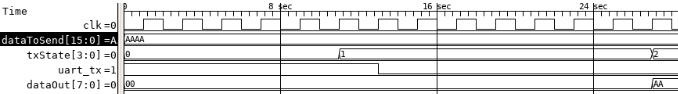
\includegraphics[width=1\textwidth ]{./images/uart_timing.png}
        \caption{UART Transmit Timing Diagram}
    \end{figure}

    \begin{figure}[H]
    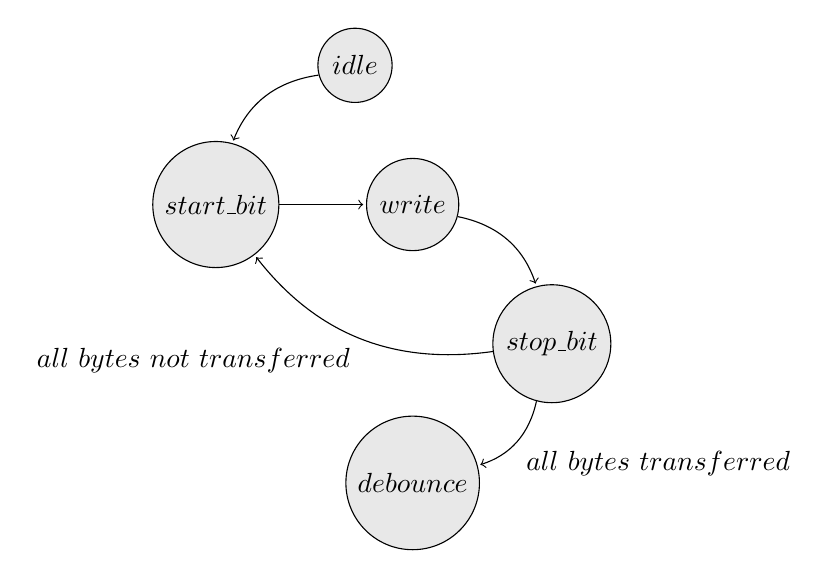
\begin{tikzpicture}[shorten >=1pt,node distance=2.5cm,auto]

    \tikzstyle{every state}=[fill={rgb:black,1;white,10}]

    \node[state]   (idle)                      {$idle$};
    \node[state] (startbit) [below left of=idle]  {$start\_bit$};
    \node[state]           (write) [right of=startbit]     {$write$};
    \node[state] (stop) [below right of=write] {$stop\_bit$};
    \node[state]           (debounce) [below left of=stop]     {$debounce$};

    \path[->]
    (idle) edge [bend right] node {} (startbit)
    (startbit) edge node {} (write)
    (write) edge [bend left] node {} (stop)
    (stop) edge [bend left] node {$all\ bytes\ not\ transferred$} (startbit)
    (stop) edge [bend left] node {$all\  bytes\ transferred$} (debounce);
    \end{tikzpicture}
    \caption{State diagram for UART Transfer Protocol} 
    \end{figure}

    UART was used for communication between Screen interface and FPGA. The screen interface contained  ESP8266 Microcontroller and a 128x32 OLED screen. 115200 was set as the baud rate between both microcontroller and FPGA.The message passed by the FPGA to screen interface is present on  \textit{Table 1} 

    \begin{table}[H]
        \footnotesize
        \setlength{\tabcolsep}{0.3em} % for the horizontal padding
        \begin{tabular}{|l|l|}
            \hline
            \textbf{UART Message}  & \textbf{Description} \\ \hline
            RECT X Y W H & build the rectangle of width W and height H on X and Y position. \\ \hline
            CIRC X Y R& build the circle of Radius R on X and Y position. \\ \hline
            PIX X Y & build the pixel on position X and Y\\ \hline
            TEXT value & Show the pixel on screen \\ \hline
            CLEAR & Clear everything on screen \\ \hline
        \end{tabular}
        \caption{UART Message sent from FPGA to Screen Interface}
    \end{table}

    \newpage

    \begin{figure}
        \centering
        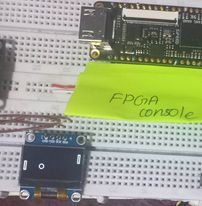
\includegraphics[width=0.3\textwidth ]{./images/uart_image.jpg}
        \caption{Screen rendering rectangle and circle element with basic screen commands }
    \end{figure}

    \subsubsection{Building the CPU}
    Building the CPU with custom instruction set architecture requires several key steps. First the requirements of the intended CPU was laid out. The required commands were finalized. According to commands, instruction set architecture was built. Discussed Instruction Set Architecture(ISA) defines 
    \begin{itemize}
        \item \textbf{Instruction Set} 

        16 Bits of word size was chosen because around 12 instructions was planned. 5 Bits out of total word size can represent all the commands as $2^5 = 32 > 12$. Other 20 bits are reserved to add other cruicial features that will support procedures, label jumping etc. The first bit is \textit{Command Modifier}($CM$) bit which signifies either the addressing mode is intermediate or not. Rest of the bits are \textit{variation} bits which either has the constant data attached to it, or signifies the variation . \textit{Table} shows how variation, commands and CM are used for Add command. 

        \begin{figure}[h]
            \centering
            \setlength{\unitlength}{0.7cm}
            \begin{picture}(16,1)
            \multiput(0,0)(0,1){2}{\line(1,0){16}}
            \multiput(0,0)(1,0){17}{\line(0,1){1}}
            \put(0,-1){\line(1,0){1}}
            \put(0,-1){\line(0,1){1}}
            \put(0,-0.7){$CM$}
            \put(1,-1){\line(0,1){1}}
            
            \put(1,-1){\line(1,0){5}}
            \put(1,-1){\line(0,1){1}}
            \put(1.2,-0.7){$COMMAND$}
            \put(6,-1){\line(0,1){1}}
            
            \put(6,-1){\line(1,0){10}}
            \put(6,-1){\line(0,1){1}}
            \put(6.2,-0.7){$VARIATION$}
            \put(16,-1){\line(0,1){1}}
            \end{picture}
            \vspace{0.4cm}
            \caption{Layout for the 16 bit Computer Word}
        \end{figure}

        \begin{table}[H]
           \footnotesize
           \setlength{\tabcolsep}{0.3em} % for the horizontal padding
           \renewcommand{\arraystretch}{1.6}
           \centering
           \begin{tabular}{|l|l|l|l|l|}
            \hline
            \textbf{Instruction} & \textbf{CM} & \textbf{COMMAND}  & \textbf{VARIATION} & \textbf{Description}\\ \hline
            ADD A & 0 & 00101 & 1000000000 & Add A to accumulator\\ \hline
            ADD B & 0 & 00101 & 0100000000 & Add B to accumulator\\ \hline
            ADD C & 0 & 00101 & 0100000000 & Add B to accumulator\\ \hline
            ADD 30 & 1 & 00101 & 000000001 & Immediate Add\\ \hline
           \end{tabular} 
           \caption{Instruction bits for Add Commands}
        \end{table}
        \newpage
        \item \textbf{Register set} 
        
         There are 5 main registers A, B ,C , Accumulator(AC) and Program Counter(PC). Initially Registers hold 0. 

        \begin{figure}[H]
            \centering
            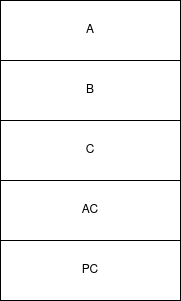
\includegraphics[width=0.3\textwidth ]{./images/registers.png}
            \caption{Registers}
        \end{figure}
    \end{itemize}

    Other essential features of the CPU are Control Unit, Arithmetic Logical Unit and other I/O devices. 

    \begin{figure}[H]
        \centering
        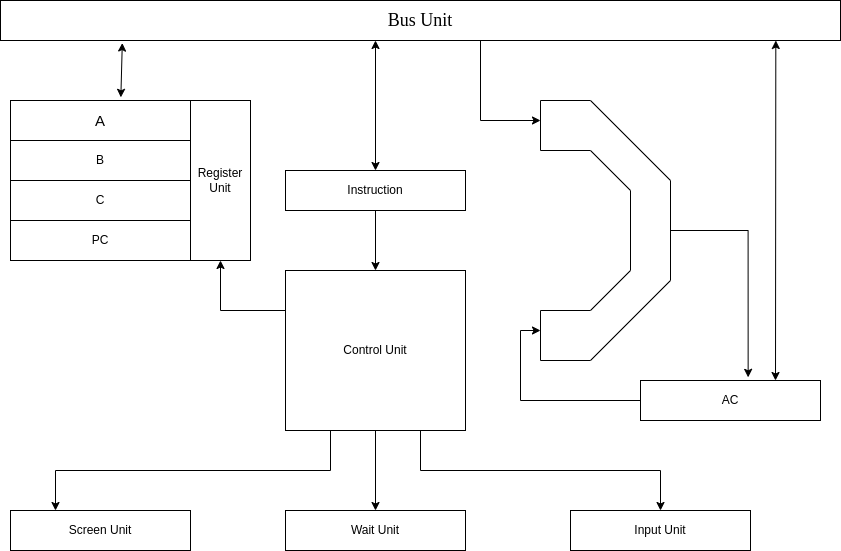
\includegraphics[width=1\textwidth ]{./images/architecture.png}
        \caption{Architecture of the CPU}
    \end{figure}

    Input Unit is constantly monitored on each clock cycle. Interrupts are not implemented to CPU polls for each input device. Screen Unit and CPU are connected with each other through the UART protocol. The functionality of control Unit state machine is shown in the \textit{Figure 13}. 

    \begin{figure}[H]
    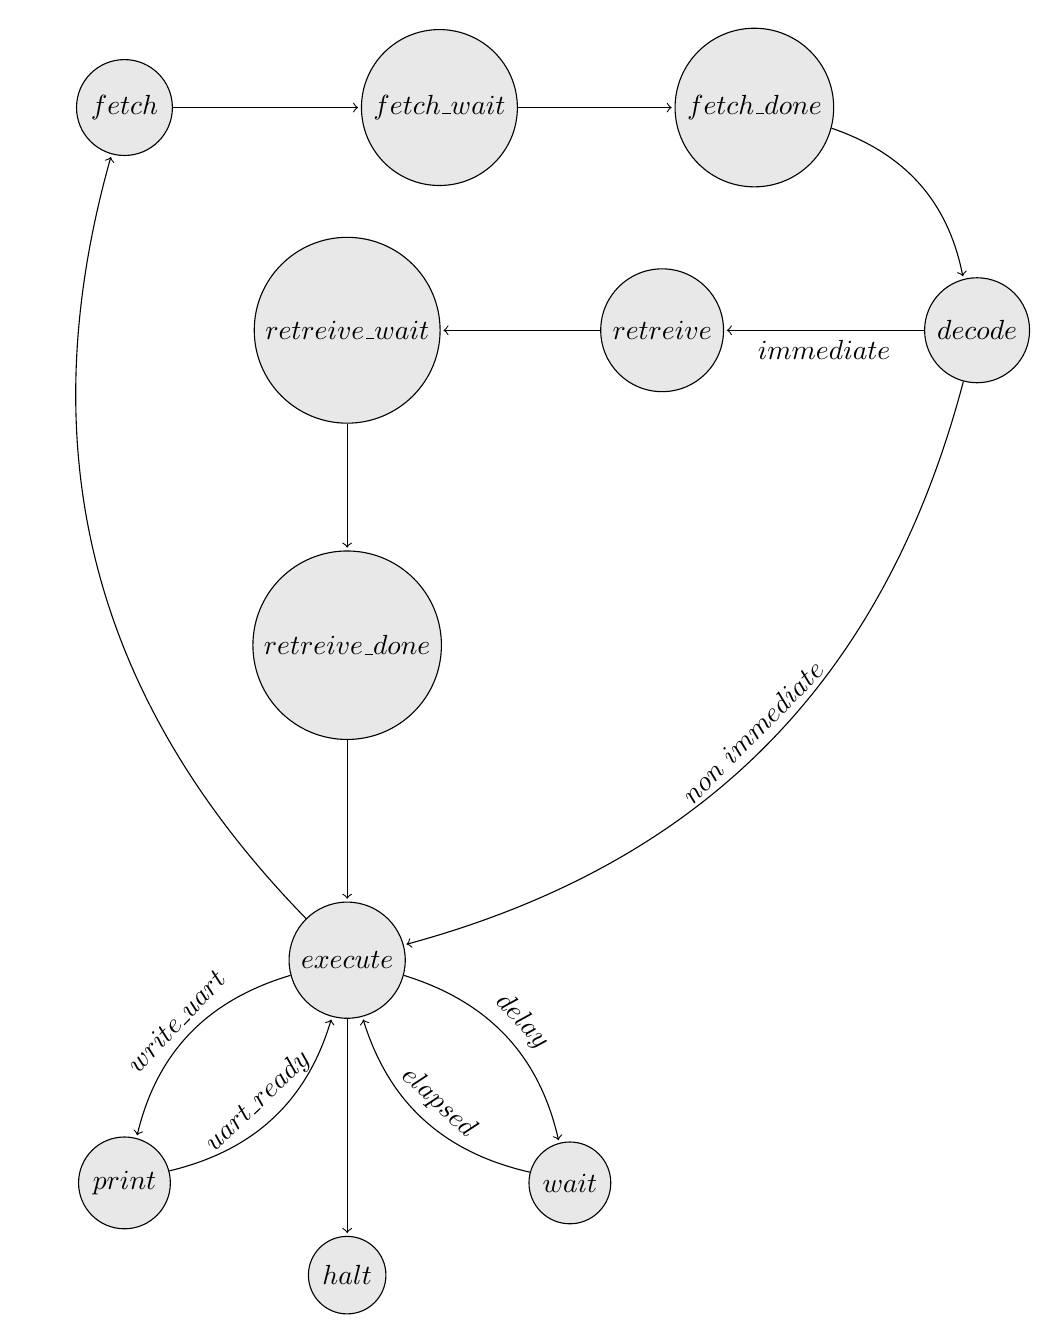
\begin{tikzpicture}[shorten >=1pt,node distance=4cm,auto]
    \tikzstyle{every state}=[fill={rgb:black,1;white,10}]

    \node[state]   (fetch)                      {$fetch$};
    \node[state] (fwait) [right of=fetch]  {$fetch\_wait$};
    \node[state]           (fdone) [right of=fwait]     {$fetch\_done$};
    \node[state] (decode) [below right of=fdone] {$decode$};
    \node[state]           (retreive) [left of=decode]     {$retreive$};
    \node[state]           (rwait) [left of=retreive]     {$retreive\_wait$};
    \node[state]           (rdone) [below of=rwait]     {$retreive\_done$};
    \node[state]           (execute) [below of=rdone]     {$execute$};
    \node[state]           (print) [below left of=execute]     {$print$};
    \node[state]           (wait) [below right of=execute]     {$wait$};
    \node[state]           (halt) [below of=execute]     {$halt$};
    \path[->]
    (fetch) edge  node {} (fwait)
    (fwait) edge  node {} (fdone)
    (fdone)  edge [bend left]  node {} (decode)
    (decode) edge  node {$immediate$}  (retreive)
    (decode) edge [bend left] node [sloped] {$non\ immediate$} (execute)
    (retreive) edge node {} (rwait)
    (rwait) edge  node {} (rdone)
    (rdone) edge  node {} (execute)
    (execute) edge [bend right]  node [sloped] {$write\_uart$} (print)
    (execute) edge [bend left]  node [sloped] {$delay$} (wait)
    (print) edge [bend right]  node [sloped] {$uart\_ready$} (execute)
    (wait) edge [bend left]  node[sloped] {$elapsed$} (execute)
    (execute) edge node {} (halt)
    (execute) edge [bend left] node {} (fetch);
    \end{tikzpicture}
    \caption{State diagram for CPU}
    \end{figure}

    CPU has total of 11 states in total. First state starts with a fetch. Other two fetch states fetch\_wait and fetch\_done are required because, reading from flash is not instantenous. The time where flash is being read represents wait time for flash and after data is read, flash has to send \textit{dataReady} signal which represents fetch\_done. Decode divides the command into \textit{CM}, \textit{COMMAND} and \textit{VARIATION} bits and checks if the instruction is immediate. If it is immediate then another 16 bit value has to be retreived which follows the same process as fetch, then it gets to execution stage. according to the instruction, it can either print, or wait, then it again goes to fetch stage.

    \begin{table}[h]
    \footnotesize
    \centering
    \setlength{\tabcolsep}{0.5em} % for the horizontal padding
    {\renewcommand{\arraystretch}{1}% for the vertical padding
    \begin{tabular}{|c|l|l|l|p{6cm}|}
    \hline
    \textbf{Command} & constant & opcode & variation & description \\ \hline
    CLEAR A & 0 & 00000 & 1000000000 & clear A Register \\ \hline
    CLEAR B & 0 & 00000 & 0100000000 & clear B Register\\ \hline
    CLEAR AC & 0 & 00000 & 0010000000 & clear AC Register\\ \hline
    CLEAR BTN1 & 0 & 00001 & 1000000000 & clear AC if btn1 pressed\\ \hline
    CLEAR BTN2 & 0 & 00001 & 0100000000 & clear AC if btn2 pressed\\ \hline
    CLEAR BTN3 & 0 & 00001 & 0010000000 & clear AC if btn3 pressed\\ \hline
    CLEAR BTN4 & 0 & 00001 & 0001000000 & clear AC if btn4 pressed\\ \hline
    STA A & 0 & 00010 & 1000000000 & store AC in A register\\ \hline
    STA B & 0 & 00010 & 0100000000 & store AC in B register\\ \hline
    STA C & 0 & 00010 & 0010000000 & store AC in C register\\ \hline
    STA LED & 0 & 00010 & 0001000000 & set first 6 bits of AC register to LED output\\ \hline
    INV A & 0 & 00011 & 1000000000 & invert A register\\ \hline
    INV B & 0 & 00011 & 0100000000 & invert B register\\ \hline
    INV C & 0 & 00011 & 0010000000 & invert C register\\ \hline
    INV AC & 0 & 00011 & 0001000000 & invert AC register\\ \hline
    HLT & 0 & 00100 & 0000000000 & halt\\ \hline
    ADD A & 0 & 00101 & 1000000000 & Add A to AC register\\ \hline
    ADD B & 0 & 00101 & 0100000000 & Add B to AC register\\ \hline
    ADD C & 0 & 00101 & 0010000000 & Add C to AC register\\ \hline
    ADD 20 & 1 & 00101 & 0000000001 & Immediate Add \\ 
    &  &  & value  & \\ \hline
    SUB A & 0 & 00110 & 1000000000 & Sub A and AC register\\ \hline
    SUB B & 0 & 00110 & 0100000000 & Sub B and AC register\\ \hline
    SUB C & 0 & 00110 & 0010000000 & Sub C and AC register\\ \hline
    SUB 20 & 1 & 00110 & 0000001010 & Immediate Subtract\\ 
    &  &  & value  & \\ \hline
    PRNT A & 0 & 00111 & 1000000000 & Print A reg to OLED \\ \hline
    PRNT B & 0 & 00111 & 0100000000 & Print B reg to OLED \\ \hline
    PRNT C & 0 & 00111 & 0010000000 & Print C reg to OLED\\ \hline
    PRNT 110 & 1 & 00111 & 0110110110 & Immediate Print value to OLED\\ \hline
    RECT X Y W H & 0 & 01000 & XXXXXYYYYY & Draw rect of in pos x and y of size w and h\\ 
    & 0 & 00000 & WWWWWHHHHH &\\ \hline 
    CIRC X Y R & 0 & 01001 & XXXXXYYYYY & Draw Circle of radius R in position X and Y\\ 
    & 0 & 00000 & 00000RRRRR & \\ \hline
    PIX X Y & 0 & 01010 & XXXXXYYYYY & Draw pixel in X and Y position\\ \hline
    JMPZ A & 0 & 01100 & 1000000000 & Jump to A Register position if AC = 0\\ \hline
    JMPZ B & 0 & 01100 & 0100000000 & Jump to B Register position if AC = 0\\ \hline
    JMPZ C & 0 & 01100 & 0010000000 & Jump to C Register position if AC = 0\\ \hline
    JMPZ 20 & 1 & 01100 & 0000000001 & Immedate jump \\ 
    &  &  & value  & \\ \hline
    WAIT A & 0 & 01101 & 1000000000 & Wait for amount of seconds as specified by A register\\ \hline
    WAIT B & 0 & 01101 & 0100000000 &  Wait for amount of seconds as specified by B register\\ \hline
    WAIT C & 0 & 01101 & 0010000000 &  Wait for amount of seconds as specified by C register\\ \hline
    WAIT 20 & 0 & 01101 & 0000000001 &  Immediate Wait for amount of seconds \\ 
    &  &  & value  & \\ \hline
    \end{tabular}
    }
    \caption{Instruction set Architecture}
    \end{table}



    \subsubsection{Writing Assembler and Assembly code}

    An assembler is a program that translates assembly language code into machine code. \textit{Table 3} contains all the possible instruction and its equivalent binary equivalent with description, which the assembler has to conver. Assembler was written in Rust which expects the filename as an argument. Each character is pushed to a dynamic array. It is then fed to the mattern matching function of rust which returns the binary executable for the CPU.

    \begin{figure}[H]
    \centering
    \lstinputlisting{pong.as}
    \caption{Pong Game Assembly Code Snippet}
    \end{figure}

    \newpage
    \subsection{System Requirement Specification}
    \subsubsection{Software specification}
    \paragraph{Verilog} 
    FPGA was programmed using Verilog HDL. It compiles the code and provides a executable which can be simulated. During simulation we can configure it so that Value Change Dump(VCD) files can also be produced.
    \paragraph{GtkWave}
    GTKWave reads the VCD files, then allows us to inspect the timing variables, which is useful for testing the usability of verilog modules.
     \begin{figure}[H]
        \centering
        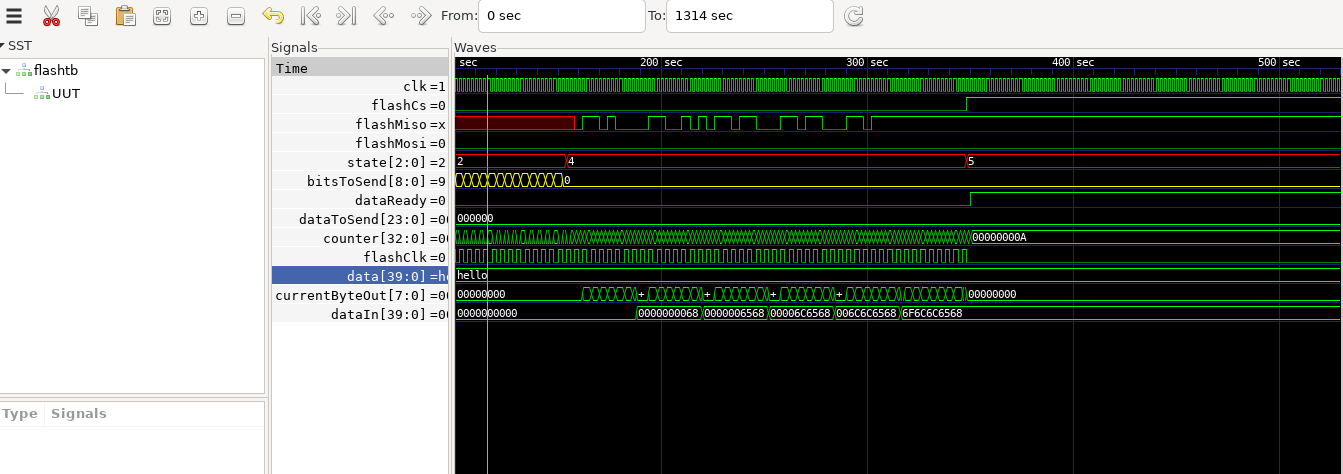
\includegraphics[width=1\textwidth ]{./images/gtkwave.png}
        \caption{Gtkwave Timing Diagram for SPI Flash}
    \end{figure}
    \paragraph{Yosys}
    Yosys is framework which synthesizes the verilog code and produces a netlist. A netlist is a file that contains the interconnections between various electric components of a circuit. So verilog code is described in digital logic form.
    \paragraph{gowitn-pnr}
    A constraint file or CST file maps the verilog variables with real pins present in FPGA. Gowin-pnr takes the constraint file then performs place and route which is suitable for Gowin FPGA.    
     \begin{figure}[H]
        \centering
        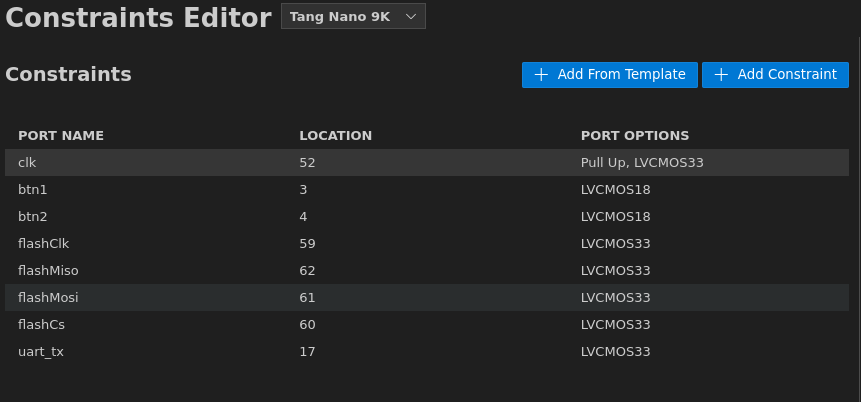
\includegraphics[width=1\textwidth ]{./images/constraint.png}
        \caption{Constraint mapping between verilog variables and the corresponding pin location}
    \end{figure}

    \paragraph{gowin\_pack}
    gowin-pack reads the output of gowin-pnr and then produces the bitstream file that is suitable to be uploaded into fpga.

    \paragraph{OpenFPGALoader}
    OpenFPGALoader is a tool to write the bitstream file into FPGA.

    \paragraph{Rust Toolchain}
    Rust is a memory safe, blazing fast language which was used to create the assembler.

    \paragraph{Espflash}
    Espflash is a tool used to flash ESP microcontroller. It was used to flash screen interface code into esp8266 microcontroller.

    \subsubsection{Hardware specification}

    \paragraph{Tang Nano 9k}
    It is open source FPGA board based on Gowin GW1NR-9 FPGA chip. It has 9k logic units, HDMI connector, SPI screen connector, SPI flash and 6 LEDs.

    \begin{figure}[H]
        \centering
        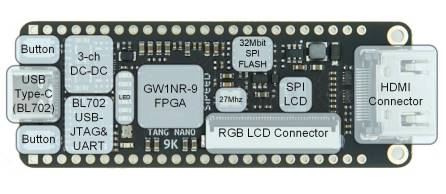
\includegraphics{./images/fpga.jpg}
        \caption{Tang Nano 9k}
    \end{figure}

    \paragraph{NodeMCU}
    It is also opensource micrcontroller board which is based on ESP8266 chip. For this project the features that were important are USB-to-UART converter and GPIO UART.
    \begin{figure}[H]
        \centering
        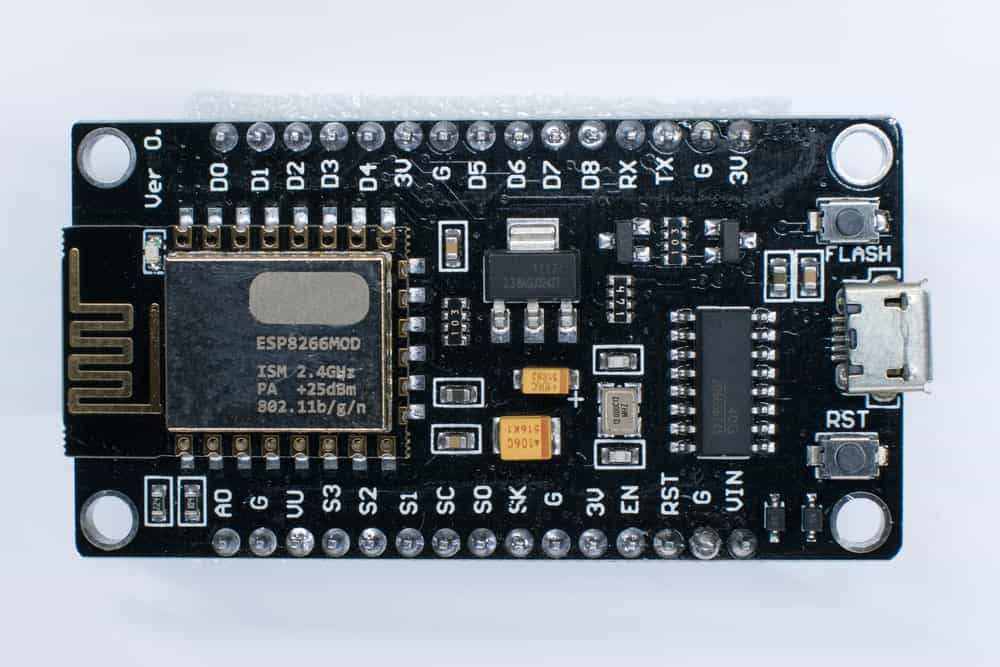
\includegraphics[width=0.5\textwidth ]{./images/nodemcu.jpg}
        \caption{Esp8266 Micocontroller}
    \end{figure}

    \paragraph{SSD1306 OLED Screen}
    It is low power consuming 128x32 pixel OLED display controller. 

    \begin{figure}[H]
        \centering
        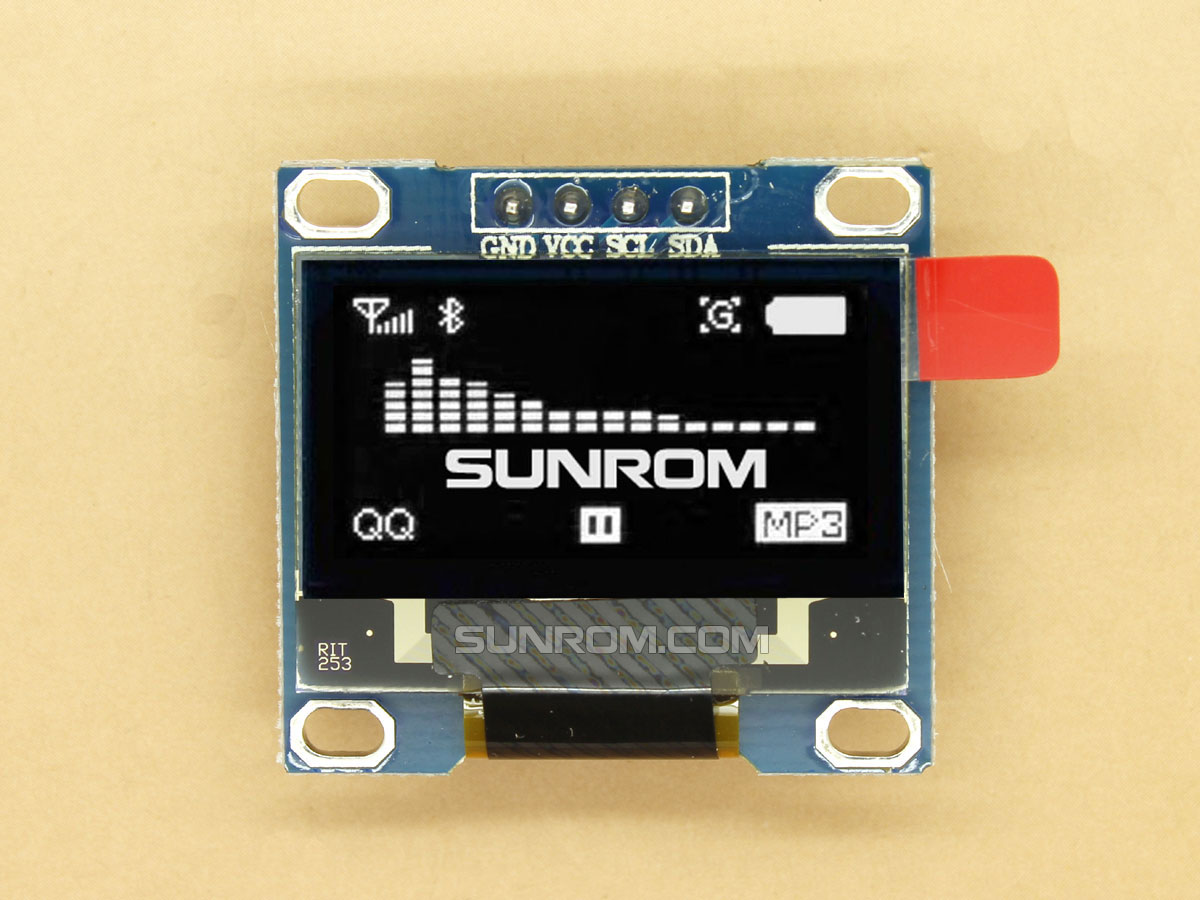
\includegraphics[width=0.5\textwidth ]{./images/ssd1306.jpg}
        \caption{OLED Screen}
    \end{figure}
    \newpage
    \section{Discussion on Achievements}

    Custom Instruction set Architecture was implemented and the functional game console was created using FPGA technology. The project also gave hands-on-experience with embedded systems. Core communication protocols like UART, SPI and I2C were also explored. Rigorous testing was done in order to find the errors on simulation phase. This project demonstrates the ability to program FPGA using open source digial design tools like Verilog, yosys, gowin-pnr etc. Other achievements include Reading Datasheets, writing simulation tests and interfacing with the device . 

    \subsection{Features}
    Some Significant features of the project are listed below

    \begin{itemize}
        \item \textbf{Custom CPU}
        \begin{itemize}
            \item RISC style CPU  
            \item 16 Bit word length 
            \item Supports up to 32 instructions
            \item Two addressing modes supported  
            \item 3 usable Registers: A, B, C
            \item 2 internal Registers : PC and AC  
        \end{itemize}
        \item \textbf{External Memory} P25Q32U is SPI supporting memory chip which is in built into FPGA itself. To load the program we can just burn the program into the flash. 
        \item \textbf{State Machine} The paradigm with which FPGA is programmed is different as FPGA supports parallelization and can run multiple blocks all at once. To take advantage of this, core modules like Flash, UART are implemented as state machine.
        \item \textbf{Uses Open source toolchains only} Sipeed also provides its own proprietary IDE, But opensource fpga tooling and documentation is very good for TANG NANO 9k. 
        \item \textbf{Communication Protocols}
        \begin{itemize}
            \item Microcontroller and OLED screen communicate with I2C protocol 
            \item FPGA and Flash communicate with SPI protocol
            \item FPGA and Microcontroller communicate with UART  
        \end{itemize}
    \end{itemize}
    \newpage
    \section{Conclusion and Recommendatation}
    The project was a great way to gain hands-on expereince with FPGA developement and custom ISA implementation. The project can be improved further by removing the limitations discussed below

    \subsection{Limitation}

    \begin{itemize}
        \item \textbf{Limited user interface/Input Device} The input device for the console consists of only 4 pushbuttons, which may not provide a rich user interface for playing games. This limits the types of games that can be played on the screen 
        \item \textbf{Non Standarized custom ISA} There are reliant and practical architectures like ARM and RISC-V which would have allowed the CPU to run already available games and the CPU would be more reliant and deterministic. 
        \item \textbf{Limited scalability} The project focuses on specific FPGA and specific OLED which means complex additions like HDMI, VGA would require significant changes to code.
        \item \textbf{Lack of Sound} Console doesn't have any audio output, which limits the gaming experience. 
        \item \textbf{Limited Memory} The size of inbuilt flash is 4 megabytes. But due to architecture limitations. only $2^{16}$ bytes can be accessed.
        \item \textbf{Display Controller} Screen Unit is managed by microcontroller, but microcontroller can be completely eliminated. Due to time constraints $I_2C$ communication couldn't be implemented in CPU. 
        \item \textbf{Cost} FPGA is versatile, and it can act as any digital circuit. The tradeoff is it's price. FPGA is good for prototype phase or for projects where ASIC fabrication price is higher than that of FPGA integration.
        \item \textbf{Limited Instruction Set} Number of instructions is very minimal which code size long and some features is not supported. 
    \end{itemize}

    
    \subsection{Future Enhancement}

    \begin{itemize}
        \item \textbf{Adding Support to more Input/Output Devices} USB support can be added which can allow range of controllers for input device. As for Output Devices we can integrate HDMI output and instead of hardcoding the screen resolution we can use clip space coordinates which will accomodate for all screen sizes. 
        \item \textbf{Adding More Games} More games can be added, and selection menu can also be added where users can select and play from range of games.
        \item \textbf{Adding Sound Support} Interactivity is very important and for that we can add sound support which makes the game more immersive 
        \item \textbf{Switch to RISC-V or ARM Architecture} Switching to such architecture allows the games to be portable. Games that are already compiled for such architecture will be able to run on the CPU itself.
        \item \textbf{Improve Performance} Currently on fetch cycle, only 16 bits is read from flash memory. Instead we can read more bytes from it.
        \item \textbf{Introduce Pipelining} Pipelining creates two different units inside the CPU. Execution unit will keep on executing and fetch unit will keep on fetching parallely, which increases the performance of the CPU.
        \item \textbf{Networking Capabilities} We can leverage chips like ESP8266 which already has implemented TCP/IP stack to create multiplayer games. 
        \item \textbf{Create Operating System} Core features of operating system like memory management, network capabilites, exceptions, interrupts and paging can be implemented. 
    \end{itemize}


    \bibliographystylebib{apalike}
    \bibliographybib{Bibliography}


    \bibliographystyleref{unsrt}
    \bibliographyref{References}
    \section{Appendix}

    \begin{figure}[H]
    \centering
    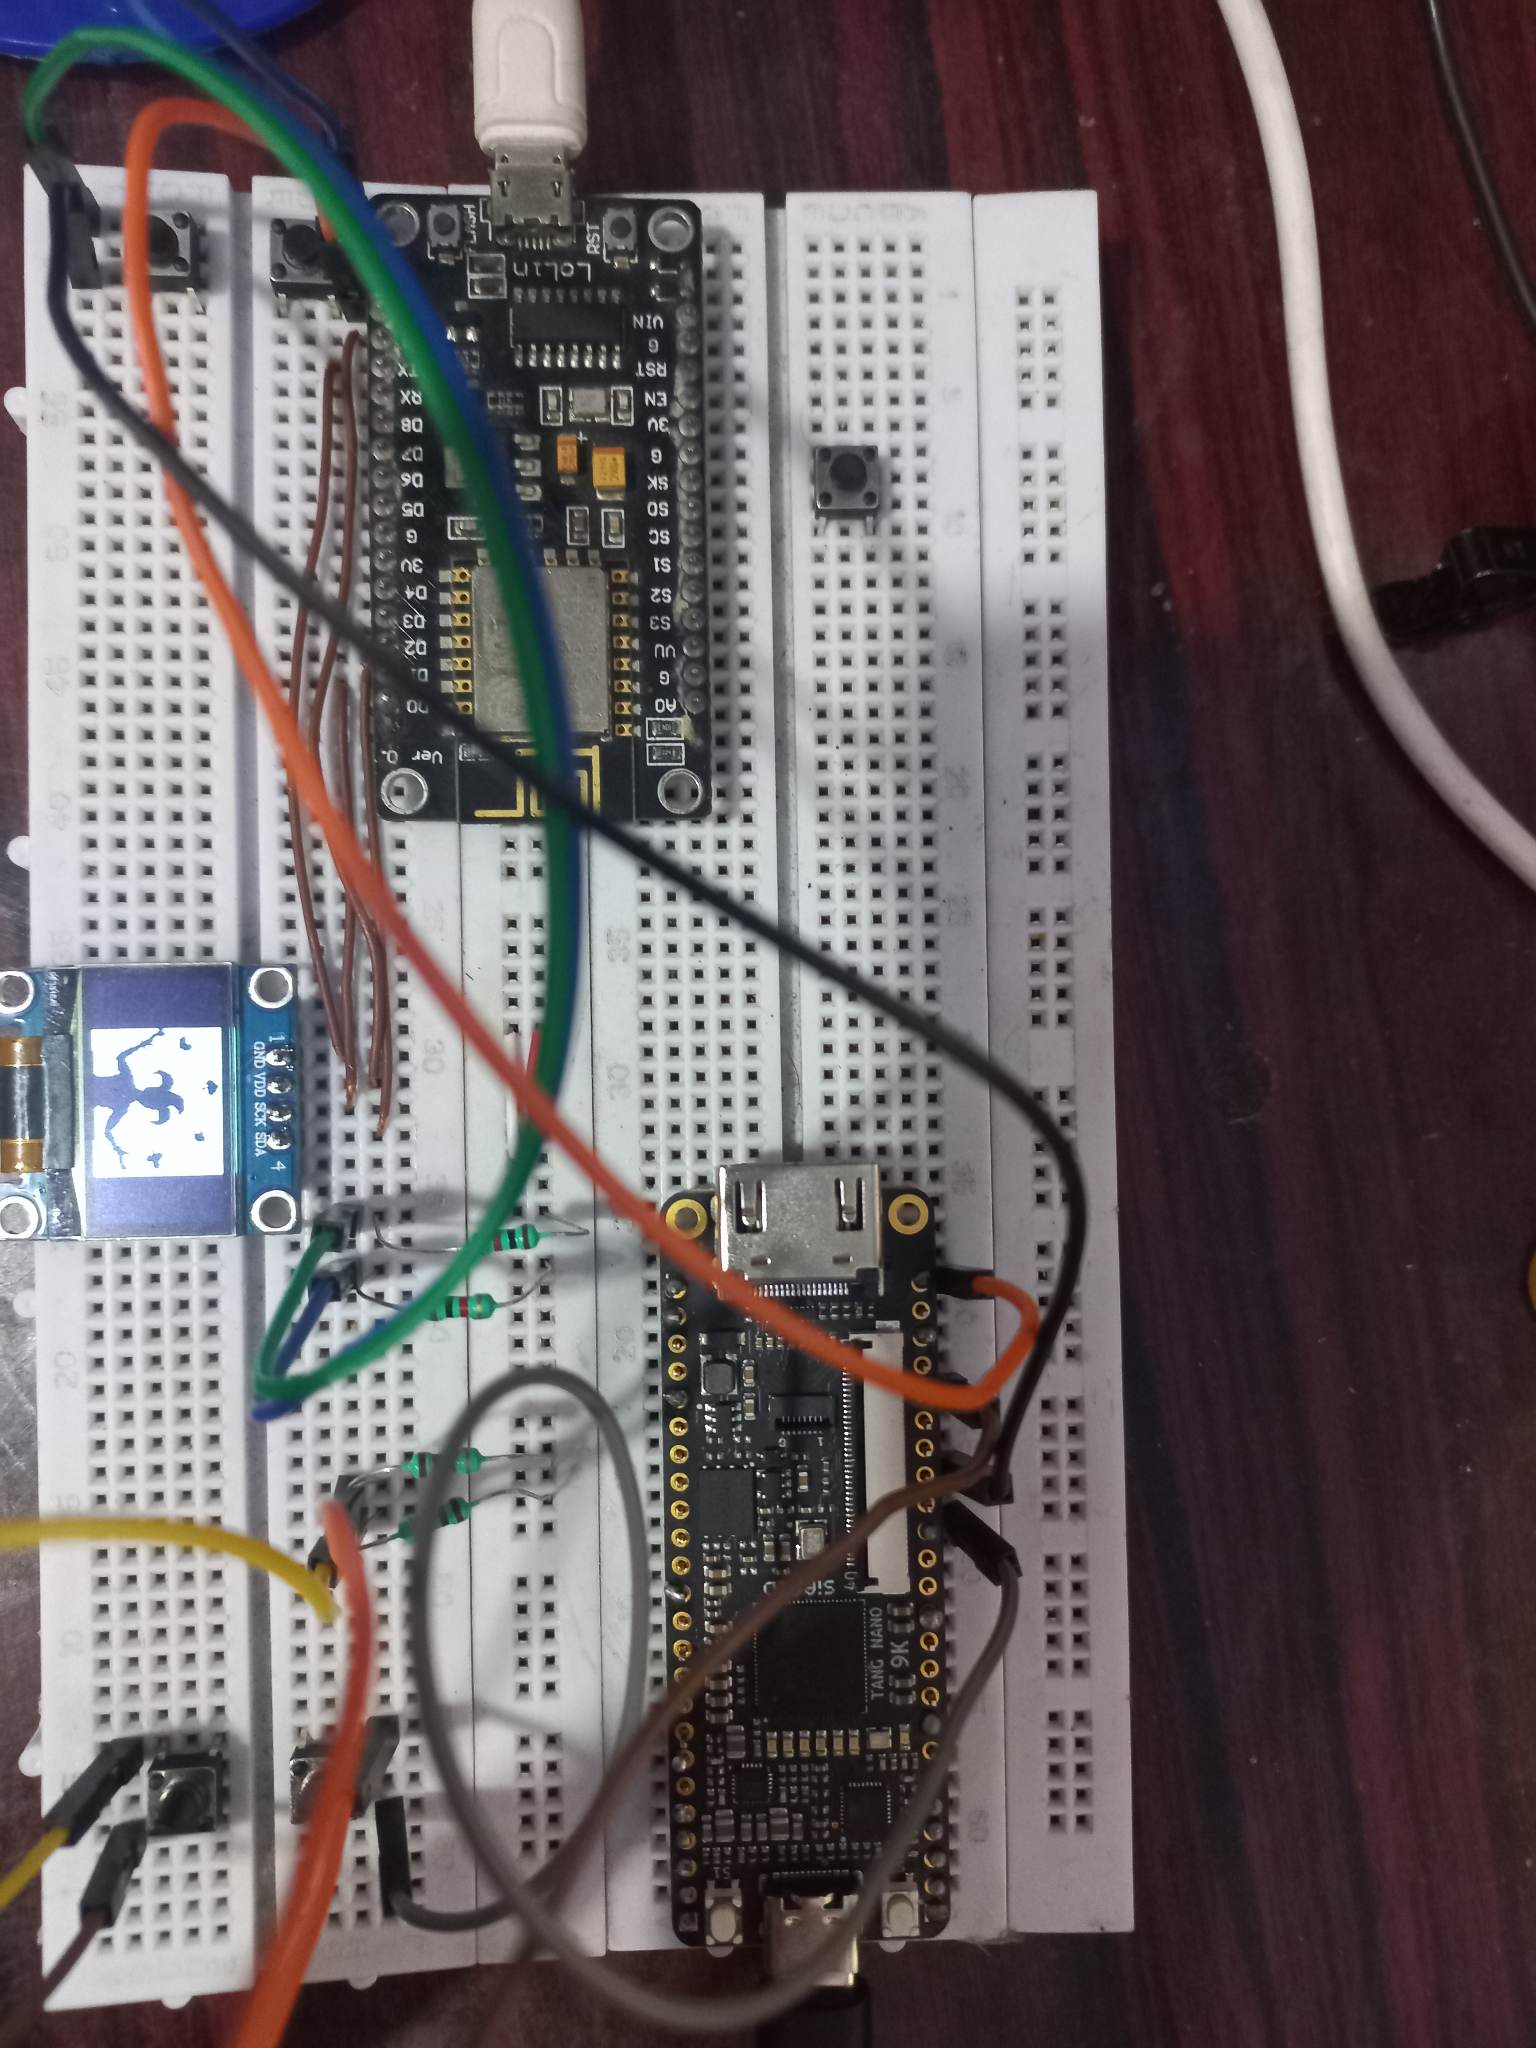
\includegraphics[width=0.8\textwidth]{images/fpga_bhoos.jpg} 
    \caption{Game Console on Breadboard}
    \end{figure}

    \begin{figure}[H]
    \centering
    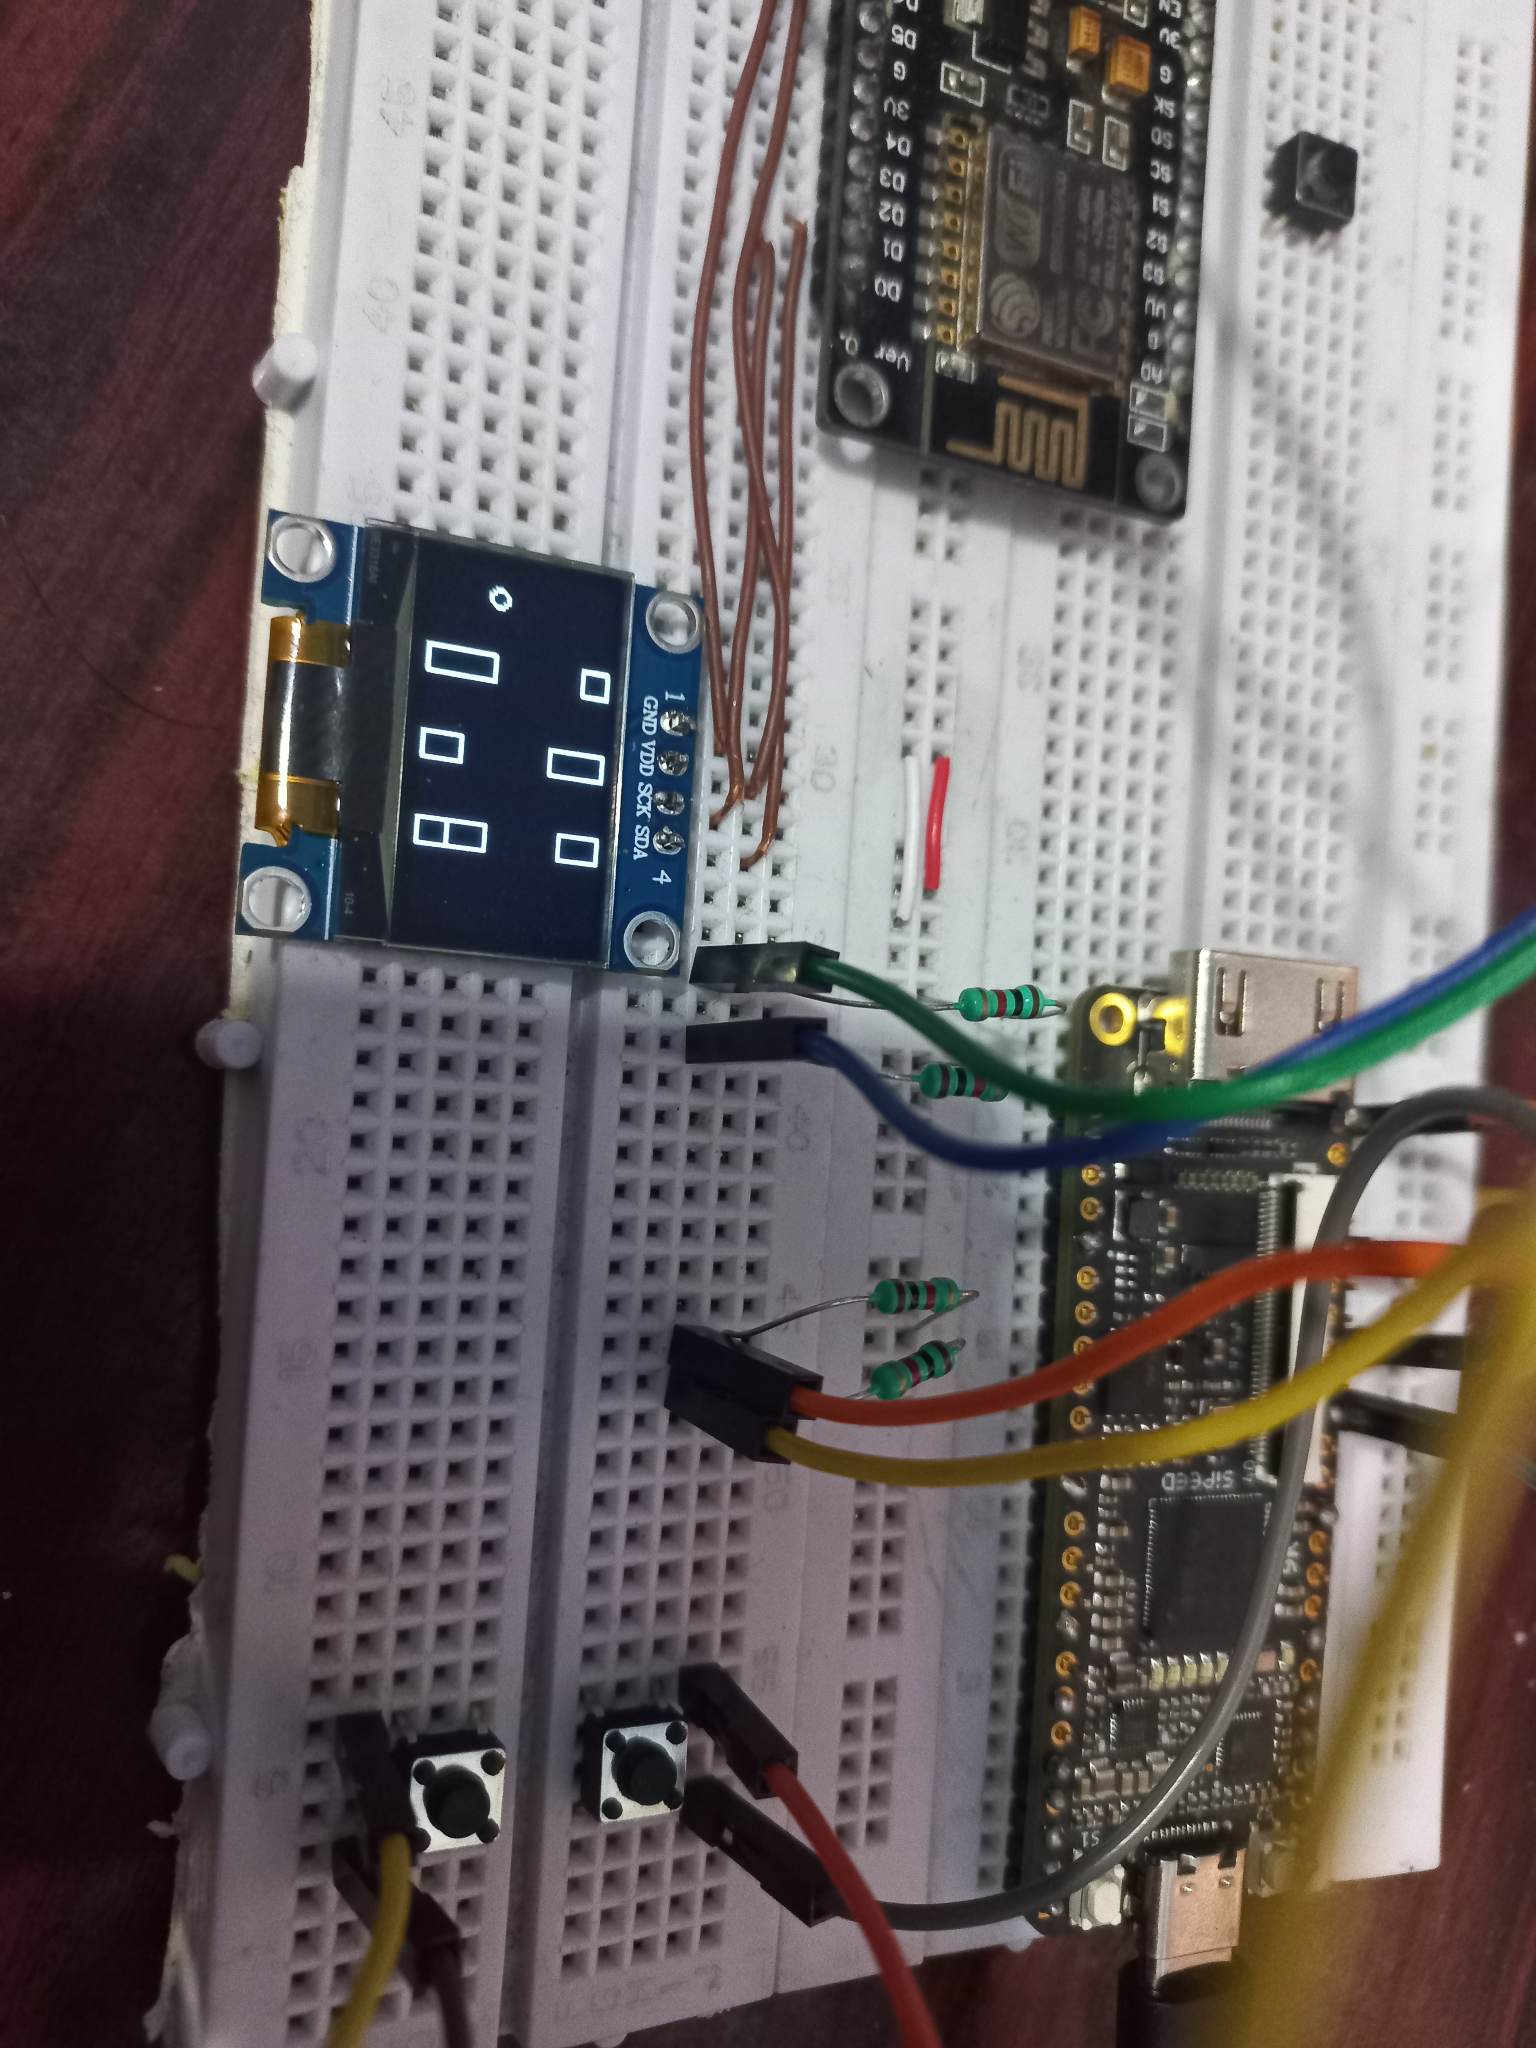
\includegraphics[width=0.8\textwidth]{images/fpga_flappy.jpg} 
    \caption{Flappy Bird style game on console}
    \end{figure}

    \begin{figure}[H]
    \centering
    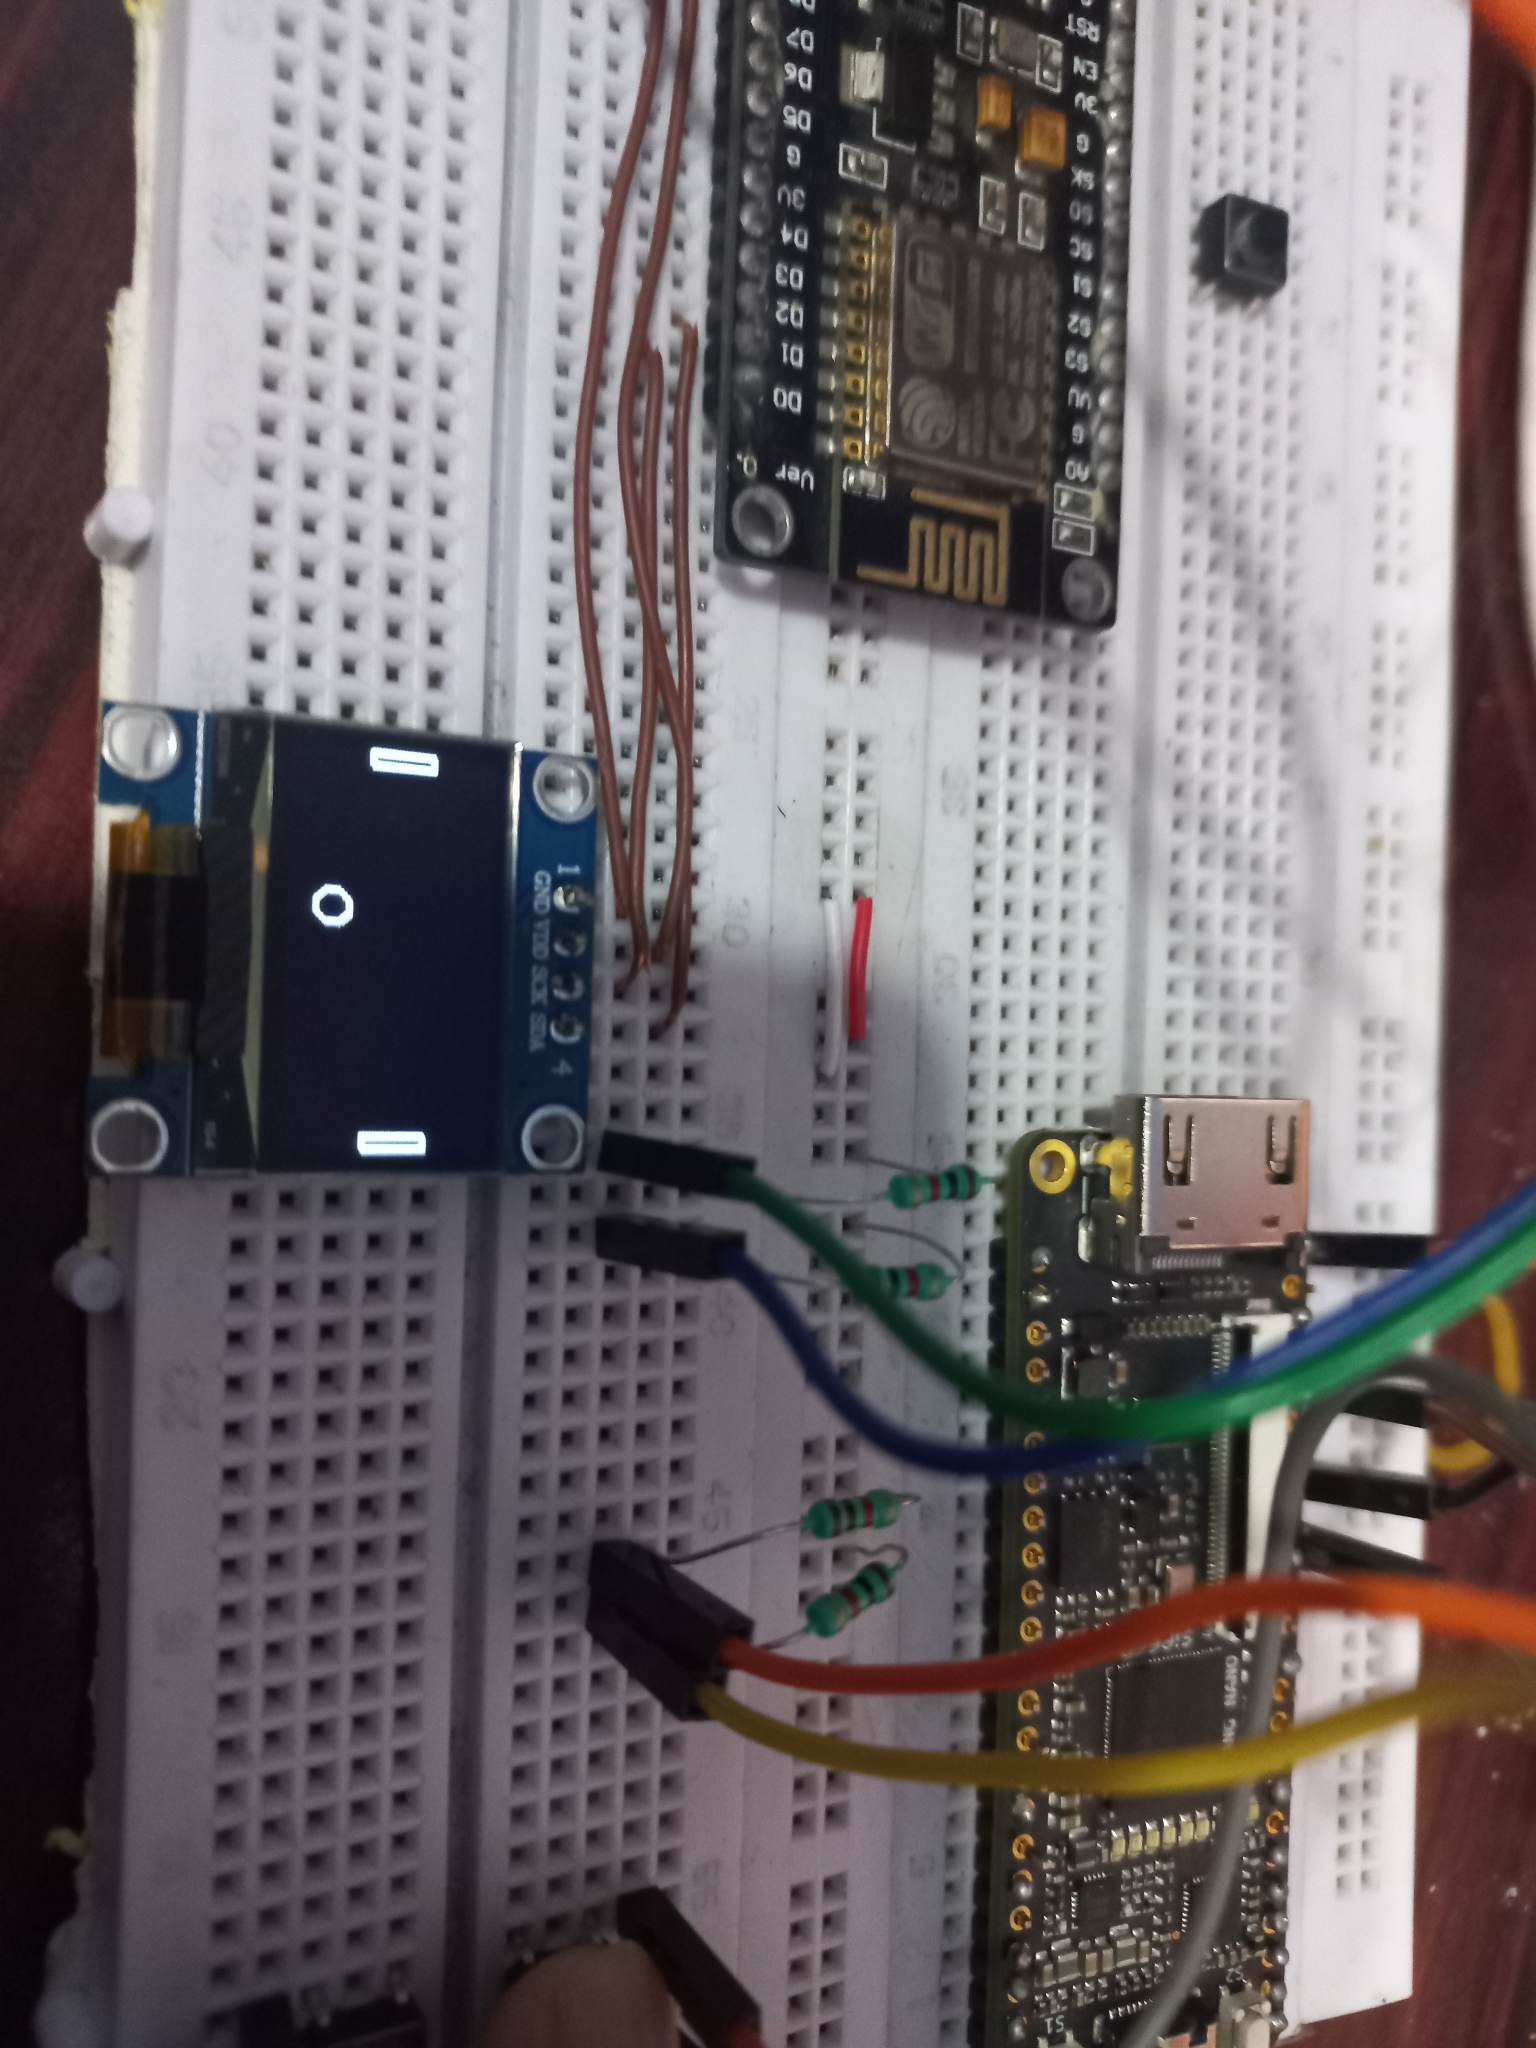
\includegraphics[width=0.8\textwidth]{images/fpga_pong.jpg} 
    \caption{Pong style game on console}
    \end{figure}
\end{document}